\section{Overview}


\subsection*{Goal}
In this assignment you will implement two offline reinforcement learning algorithms: Implicit Q-Learning and Conservative Q-Learning. You'll be experimenting with different hyperparameters and offline datasets that have been provided to you. Data collection is one of the most practical problems with applying Deep RL, and it's a common practice to try different exploration strategies for a given problem. In this assignment, we provide you with Random $\mathcal{E}$-Greedy and Random Network Distillation based exploration strategies for you to compare the quality of the collected data.


You will then have the opportunity to train and tune these agents in a variety of environments in the Simple PointMass physics simulator. We provide the code for generating the offline datasets as part of the assignment. Your objectives are as follows:

\begin{enumerate} 
    \item Implement and train the Implicit Q-Learning and the Conservative Q-Learning algorithms for Offline Reinforcement Learning.
    \item Experiment with the key hyperparameters for each algorithm and explore how they affect performance of your RL agents.
    \item Analyze differences between the quality of different offline data samples provided to you. 
\end{enumerate}

Notice that implementing algorithms may take longer time to finish than analyzing the results.


\subsection*{Codebase}
 We provide you with offline transitions dataset $\mathcal{D}$. Assuming your replay buffer has been populated with the offline dataset trajectories, your goal is to implement the corresponding reinforcement learning algorithms.

For each problem, we provide you with the files that you need to complete. Sections that need to be filled have been marked with \texttt{TODO} tags.


\vspace{0.2cm}

\noindent\textbf{Use of GPT/Codex/Copilot/Any AI code assistant/agent:} For the sake of deeper understanding on implementing imitation learning methods, assistance from generative models to write code for this homework is prohibited. 

You will submit the entire \texttt{submission} directory. To do so run the command  below from the \texttt{src} directory

\begin{verbatim}
    bash collect_submission.sh
\end{verbatim}

or you can choose to zip the folder up manually.

\newpage

\subsection*{Preliminaries}

\paragraph{Environments: } In this assignment, we'll be working with the Pointmass environment. 

The goal for the Pointmass environment is to navigate a gridworld of varying difficulties: \texttt{easy, medium} and \texttt{hard} to reach the ``goal'' location. Sample environments for each difficulty have been visualized in Figure \ref{fig:pointmass_vis}

\begin{figure}[htbp]
    \centering
    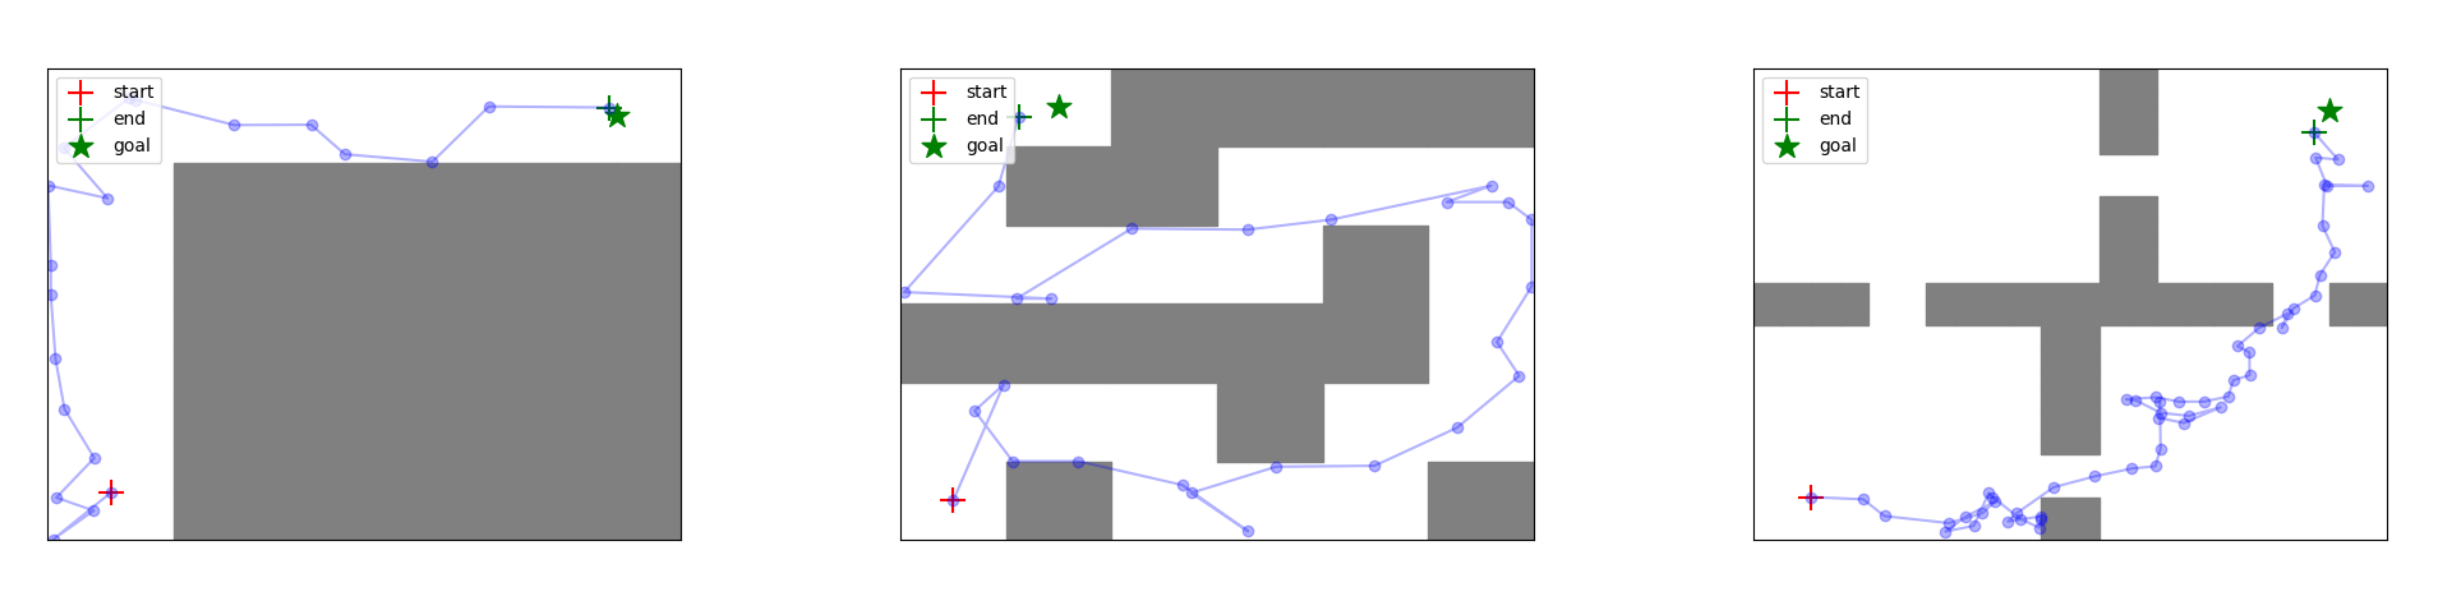
\includegraphics[scale=0.38]{figures/point_mass_envs.png}
    \caption{Visualization of the Point mass environment with varying difficulty levels for navigation and reaching the goal.}
    \label{fig:pointmass_vis}
\end{figure}


\paragraph{Offline datasets: } For offline RL, we have provided you with a set of exploration strategies which are used to populate the replay buffer. These trajectories then serve as the training dataset for your offline RL algorithms. In this assignment, you'll experiment with two exploration strategies (i) a Random $\mathcal{E}$-Greedy strategy and (ii) \href{https://arxiv.org/abs/2110.06169}{Random Network Distillation (RND)} algorithm. 

The RND algorithm, aims at encouraging exploration by asking the exploration policy to more frequently undertake transitions where the prediction error of a random neural network function is high. Formally, let $f_\theta^*\left(s^{\prime}\right)$ be a randomly chosen vector-valued function represented by a neural network. RND trains another neural network, $\hat{f}_\phi\left(s^{\prime}\right)$ to match the predictions of $f_\theta^*\left(s^{\prime}\right)$ under the distribution of datapoints in the buffer, as shown below:

\begin{equation}
    \phi^*=\arg \min _\phi \mathbb{E}_{s, a, s^{\prime} \sim \mathcal{D}}[\underbrace{\left\|\hat{f}_\phi\left(s^{\prime}\right)-f_\theta^*\left(s^{\prime}\right)\right\|}_{\mathcal{E}_\phi\left(s^{\prime}\right)}]
\end{equation}

If a transition $(s,a,s^\prime)$ is in the distribution of the data buffer, the prediction error $\mathcal{E}_\phi(s^\prime)$ is expected to be small. On the other hand, for all unseen state-action tuples it is expected to be large. To utilize this prediction error as a reward bonus for exploration, RND trains two critics – an exploitation critic, $Q_R(s,a)$, and an exploration critic, $Q_\mathcal{E} (s, a)$, where the exploitation critic estimates the return of the policy under the actual reward function and the exploration critic estimates the return of the policy under the reward bonus. In practice, we normalize error before passing it into the exploration critic, as this value can vary widely in magnitude across states leading to poor optimization dynamics.


\newpage